% $Id: AllegProposal.tex,v 1.8 2000/07/05 21:02:12 culver Exp $
% AllegProposal.tex
% by A. Thall
% 13. Feb 2003
%
% Small edits and a few additions made by R. Roos
% 21 Jan 2007
% Most particularly, the "box" around the thesis statement has been removed,
% section titles have been modified. The section named "Prior work II" has
% been commented out. The \topmargin has been changed to -.5in and the
% change to \parindent has been commented out.
% The filename "nausicaa.eps" has been changed to simply "nausicaa" so that
% pdflatex can be used on the file (and a file named "nausicaa.pdf" has
% been created using the "epstopdf" command).
% Several subsections have been added to illustrate subsection usage.
% The word "comp" has been replaced by "project" or "thesis" throughout.
% Other small changes have been made.
%
% This document provides a sample Senior Project Proposal template for use
% by students in Allegheny's CS and Applied Computing programs.

\NeedsTeXFormat{LaTeX2e}
\documentclass[11pt]{article}

%The following is used by WinEdt to set up cross-referencing to the BibTeX files
%It is NOT commented out---the comment lets it be simply ignored by non-WinEdt LaTeX compilers

%GATHER{mybibtexDB.bib}

\usepackage{setspace}
\usepackage{amsmath}
\usepackage{amssymb}
\usepackage{epsfig}
\usepackage{fancybox}
\usepackage{listings}
\usepackage{algo}
\usepackage{url}

%----------My added Packages-----------------
\usepackage{soul}
\usepackage{graphicx}
\usepackage{amsthm}
\newtheorem{ProposalDef}{Definition}
\usepackage{color}
\newcommand{\hilight}[1]{\colorbox{yellow}{#1}}

\usepackage{titlesec}
\titleformat{\subsubsection}[runin]{\normalfont\bfseries}{}{}{}[]

\soulregister{\em}{1}
%-------------------------------------------------------

\setlength{\textheight}{9in}
\setlength{\textwidth}{6in}
\setlength{\oddsidemargin}{.25in}
\setlength{\topmargin}{-.5in}  % changed from -.25 by RSR on 1/21/07
%\parindent .5in    % commented out by RSR 1/21/07

%put words in the hyphenation statement if you want to enforce
%how LaTeX should break them (or not) at the end of a line.
%\hyphenation{repre-sen-tations problems exact linear}
\hyphenation{itself}

%%%%%
%% Commented out -- RSR, 1/21/07
%%%%%
% The following provides a box to surround the thesis statement
%\newenvironment{Thesis}%
%{\begin{Sbox}\begin{minipage}{.95\linewidth}}%
%{\end{minipage}\end{Sbox}\begin{center}\fbox{\TheSbox}\end{center}}

\title{Incremental Model Synchronization in Model Driven Engineering}
\author{Hamid Gholizadeh \\ Supervisor:  Dr. Tom Maibaum \\ 
Committee Members: Dr. Wolfram Kahl, Dr. Jacques Carette }

\begin{document}

% You can specify a language and other options for
% the code-formatting "listings" package
\lstset{language=C++,basicstyle=\small,
        stringstyle=\ttfamily,showstringspaces=false}

\singlespace
\maketitle

\begin{abstract}                % ~350 words max
Abstract parts goes here.
\end{abstract}

\doublespace
% This sets section-numbering to only include Section and Subsection numbers
\setcounter{secnumdepth}{2}

\section{Introduction(general introduction starting from MDE to reaching Synchronization goes here: Synchronization Definition, demostrate its importance by giving example from Software development, you can refer to Landscape of bidirectional model synch ...}\label{ch:overview}

MDE (Model Driven Engineering) is proven to be a demanding approach in software development process \cite{Brambilla:MDE:2012dq,Bezivin:MDA:2004nx}. One of the intentions of the MDE approach in Software Development is to bring the intelligence of the human being to the more abstract level of models rather than concrete level of the codes. In Model Driven Software Engineering (MSDE), models are to be considered as active and first-class citizens of the software engineering process artifacts as opposed to the current practice where models --like UML diagrams-- are usually used as a supportive and rather passive artifacts, e.g. for software development team inter-communications. The latter happened because of the lack of complete formality and tool support for maintaining models; for example {\em Model Management} as a core task of MDE, still lacks enough formal foundation and applicable tools, supporting its demanded functionalities like {\em Model Correspondence Specification} and its maintenance in terms of {\em Model Synchronization} or {\em Change Propagation},  and {\em Conflict resolution.} 
There are still many research at the moment on some other aspects of {\em Model Management} like {\em Model Transformation} which is discussed in the Section \ref{sec:Lit} in more details.

In a typical practice of software engineering process, models are evolving  form more abstract levels to more concrete levels of the code. we call this process {\em model refinement} and can look at it like vertical movement from more abstraction to less abstract levels. This {\em Vertical} movement usually needs to be taken in a reverse direction which is also called {\em reverse engineering}-- to fit and accomplish in the iterative method of software development process, where it is called {\em round-trip engineering}. During round-tripping process, sometimes it is necessary to move between the models at the same levels of abstraction --movement not changing the level of abstraction, Therefore it is called horizontal movement as apposed the latter vertical movement. That is, like the previous case can be in a forward and backward direction (Figure  \ref{fig:model-code}.)

%:Key private-shared Picture
 \begin{figure}[ht!]
\centering
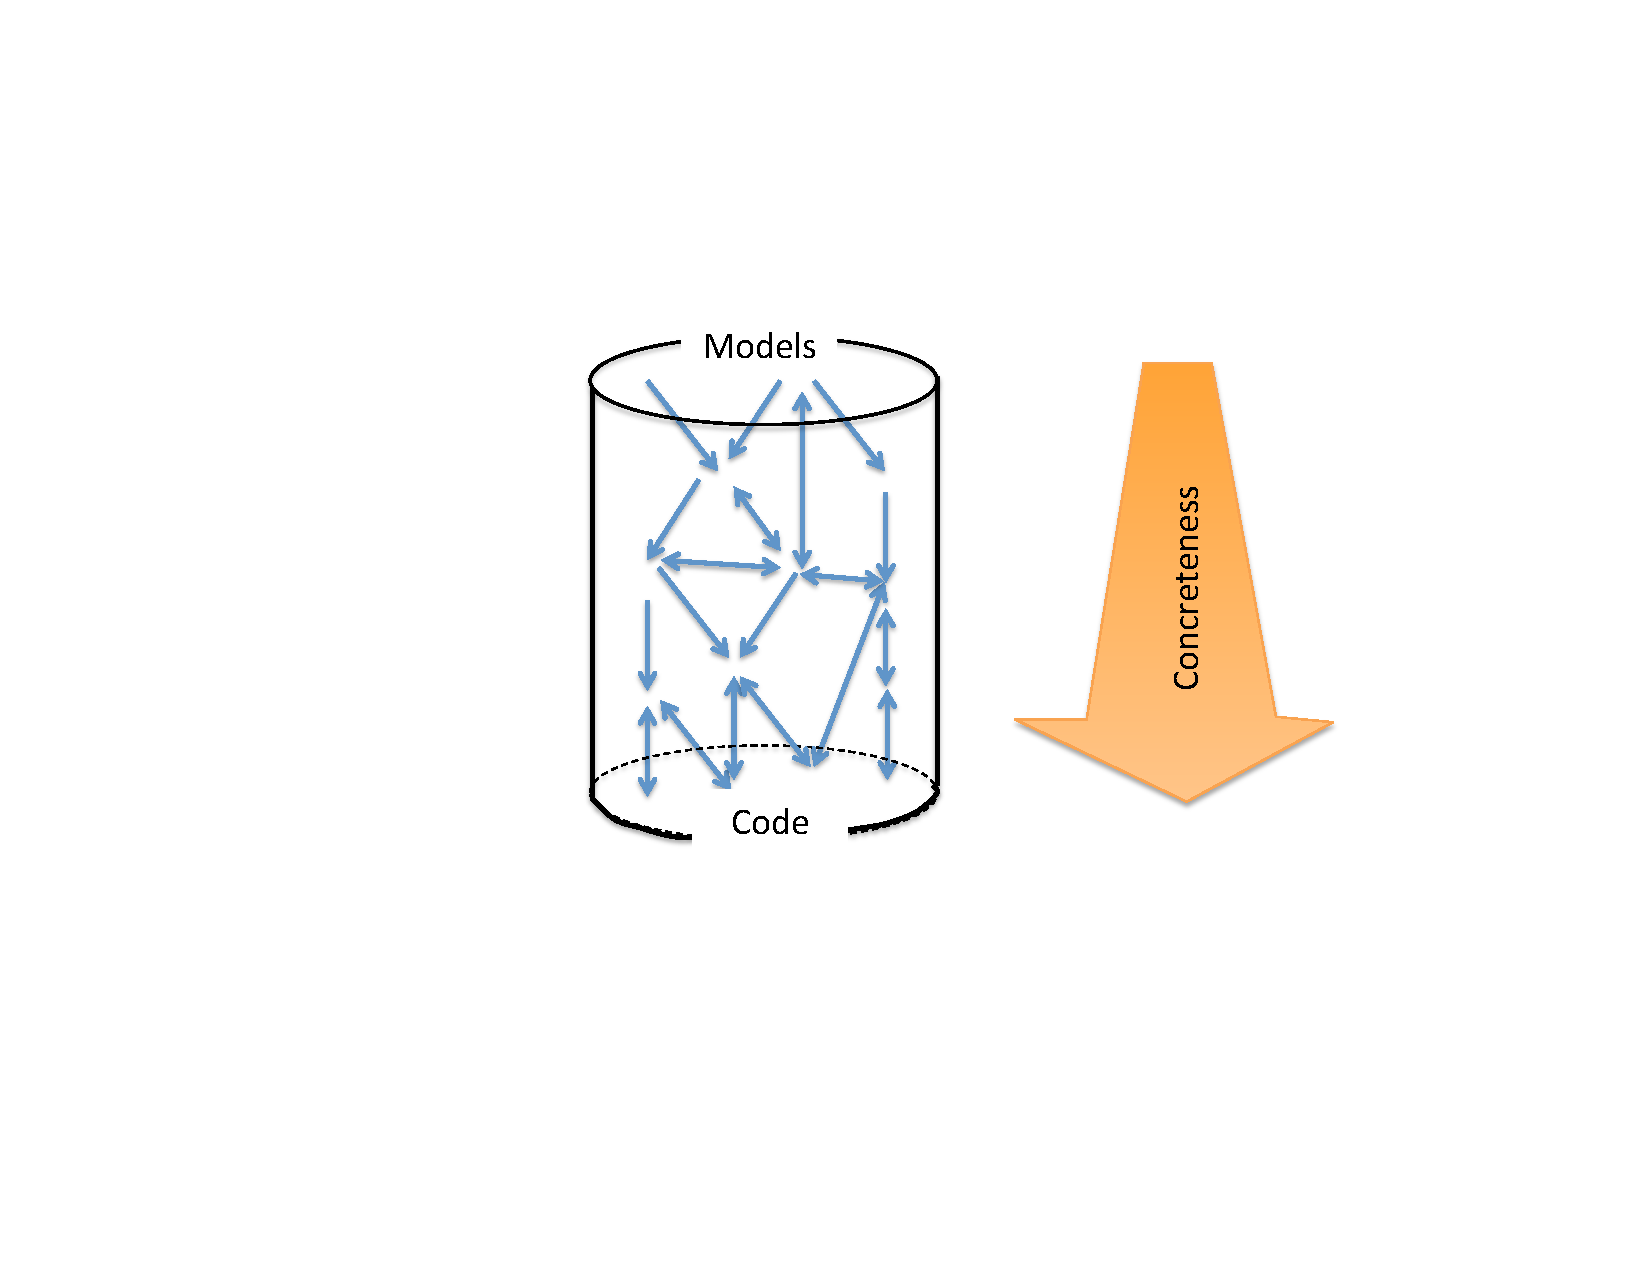
\includegraphics[width=50mm]{images/model-code}
\caption{Vertical and horizontal movements in software eng.}
\label{fig:model-code}
\end{figure}


The horizontal movement is because each model might demonstrate and focuse on different aspects of the software system, or maybe some models are suitable for different users to work with. For example, in a typical development process of software development using UML diagrams(Models,)\footnote{we consider a diagram as a model, but not the other way around, i.e. models not need to be diagrammatic.} each model share some common parts with other models and some have their own specifics feature. E.g. {\em Class Diagram} and {\em State Chart} diagram can share some of the class method signature, while attribute names for the classes, and the order of the events happening are consequently considered as a specific(private) part of each.

Because of the inevitable changes which is frequently happing during the software development process, and also during the maintenance phase \cite{Briand:UMLChangeMng:2013cr}, it is necessary to handle the {\em change propagation} which is actually is the semantic of the ``movement'' in previous paragraph. Hence change propagation can happen {\em Vertically} or {\em Horizontally}. By {\em Vertical} change propagation we mean a Model {\em refinement} from more abstract level to more concrete one or vice versa. By {\em Horizontal} refinement we mean change propagation among the models, since they are sharing some concept together as discussed in previous paragraph. Taking software artifacts a models, industrial projects would include hundreds or even thousands of artifacts which are inter-related to each other in some ways, so changing one artifact would require change propagation throughout the whole system. Handling this situation by user without a tool support even in small scale is tedious, complicated, error-prone and very time consuming and for the large cases is nearly impossible. That is why nowadays, much emphasis is put on the code rather than a model, which made Software Engineering deprived of many proved benefit of Model Driven Software Development. Ending up with the inconsistent artifacts of the software development is the typical story of the large scale software projects which most of them are usually looked as a outdated historical record and rather as a decorative pieces than the live and valuable software entities 
%{\em Software artifacts other than code is so important that \cite{Fundamental of Information Technology} defines software as a programming code plus the modelling artifacts and documentations.} 

This thesis proposal examines underlying formalities and existing works in the area of  {\em Model Synchronization} and identifying some gaps in current works and motivates how addressing those gaps is necessary in specification and implementation of formal synchronization framework, since it  would provide formal foundation for verifying the implemented synchronization framework. To be more specific we intend to address the formalities underlining the {\em Shared} and {\em Private} parts of the related models which matters in {\em Model Synchronization}. More detailed discussion on the problem is covered in section \ref{sec:Problem}. We will also discuss briefly some other  open problems, including {\em Concurrent Model Synchronization} and {\em Conflict Resolution} strategies $-$ which might  be an extended work of this research, that we observed during the survey on {\em Model Synchronization} area for future reference.

\hl{You can put some examples here as an introduction of the case.}

\hl{You need to define  Model Synchronization somewhere}


\section{Background :some backgrounds goes here, from the definition of model
formally, what is ATG, what is meta-model, What is State-based lenses, what is delta-base, 
what is Graph Grammer, Synchronization Properties : Correctness, Completeness, Hipocraticnes, Heridatiry and .... }

By \textbf {Synchronization}  we mean reconstructing the {\em Relation} between two {\em Models.} These two models already might have been in a consistent state, i.e. are related by R, or might be newly created models which consistency was not established between them yet. Models formally can be represented as an Attributed Types graph \cite{Ehrig:2004:FundementalATG, book:Ehrig2010}.  We are going to define some basic definitions regarding the formal foundation of Models in the following. These definition are adapted from \cite{book:Ehrig2010, Ehrig:2004:ATGFundemental}


\subsection{Model as an Typed Attributed Graph}
In general a Model can be represented as a Graph which consist of a nodes and edges connecting these nodes. e.g. a Class diagram in UML is a graph with classes as a node and the associations between the classes as a node. Since we need a richer structure than a simple graph we need to extend the formality of a graph to make it possible to capture further values annotated to the nodes and edges, Hence Attributed Graphs are introduced. Attributed graph are like ordinary graph extended in a way that for every {\em Node} and {\em Edge}, it is possible to introduced a Data called  {\em Attribute} and bind that by an edge called {\em Attribute Edge} to corresponding Nodes and Edges. So, first we need to extend the concept of regular graph to make it possible for the edges to have outgoing edges like nodes. This extended version of graphs is called {\em E-Graph} and introduced in the following.


%:Key Def1(E-graph G)
\begin{ProposalDef}
An \textbf{E-graph G} is defined as $G=(V_G,E_G, V_D, E_{NA},E_{EA} ,(source_j$ $,target_j)_{j \in \{G,NA,EA\}) }$
\begin{itemize}
	\item $(V_G,E_G,source_G,target_G)$ constitutes a regular Graph with $V_G$ as Nodes, $E_G$ as Edges and $source_G$ and $target_G$ as source and target functions  respectively.
	\item $V_D$ is a Data Nodes
	\item $E_{NA}$ and $E_{EA}$ are called Node Attributes and Edges Attributes, which are connecting respectively $V_G$  and $E_G$ to $V_D$. 
	\item source and target functions are defined as below:
	\begin{itemize}
		\item $source_G : E_G \rightarrow V_G$, $targetG : E_G \rightarrow V_G$;
		\item $source_{NA} : E_{NA} \rightarrow V_G$, $target_{NA}: E_{NA} \rightarrow V_D$;
		\item $source_{EA} : E_{EA} \rightarrow E_G$, $target_{EA}: E_{EA} \rightarrow V_D$;
	\end{itemize}
\end{itemize}

\end{ProposalDef}

%:Key Def2(morphism between E-graphs)
\begin{ProposalDef}

\textbf{morphism between E-graphs} $G^1$ and $G^2$ with 
$G^k = (V_G^k, V_D^k, E_G^k, E_{NA}^k$ $,E_{EA}^k, (source_j^k, target_j^k)_{j \in \{ G, NA, EA \}})$ for $k = 1, 2$ is defined as $f:G^1 \rightarrow G^2$ which is a tuple $(f_{V_G},f_{V_D},f_{E_G},f_{E_{NA}},f_{E_{EA}})$ 
with $f_{V_i} : V_i^1 \rightarrow V_i^2$ and  $f_{E_j} : E_j^1 \rightarrow E_j^2$ for $i \in \{G,D\}$, $j \in \{G,NA,EA\}$ such that $f$ commutes with all source and target functions, for example $f_{V_G}  \circ source_G^1= source_G^2 \circ f_{E_G}$

\end{ProposalDef}

%:Key Def3(Category EGraphs)
\begin{ProposalDef}
E-graphs and E-graph morphisms form the \textbf{Category EGraphs}.
\end{ProposalDef}

 {\em Attributed Graphs} are Graphs that is accompanied by a Data Algebra in a sense that the Data Nodes are taken from the subset of algebra {\em Carrier sets}. To be more precise, we first distinguish a subset of a Carrier set of an algebra and consider the contents of each member in this subset as a {\em Data Node}. In graphical illustration of the Attributed Typed Graph we ignore those {\em Data Nodes} that are not reachable from the underlying Graph Nodes and Edges. See an example in \cite{book:Ehrig2010} for more details.
  
%:Key Def4 (Att Graph Def)
\begin{ProposalDef}
Let $D_{SIG} = (S_D,OP_D)$ be a data signature with attribute value sorts $S_D$ and operations $OP_D$ and take $S'_D \subseteq S_D$. An \textbf{Attributed Graph(AG)} $AG = (G,D)$ consists of an E-graph $G$ together with a $D_{SIG}$-algebra $D$ such that $V_D$ is disjoint union of the selected carrier sets, i.e. $V_D=\overset{\centerdot}{\cup}_{s \in S'_D} D_s$ where $D_s$ is coresponding carrier set of s.
\end{ProposalDef}

%:Key Def5 (Att Graph Morphism )
\begin{ProposalDef}
an \textbf{Attributed Graph Morphism}  $f : AG^1 \rightarrow AG^2$ for two AG graphs $AG^1=(G^1,D^1)$ and $AG^2 = (G^2,D^2)$ is a pair $f=(f_G,f_D)$ with an E-graph morphism $f_G : G^1 \rightarrow G^2$ and an algebra homomorphism $f_D : D^1 \rightarrow D^2$ such that diagram (1) commutes for all $s \in S'_D$, where vertical arrows are inclusions:

\begin{figure}[ht!]
\centering
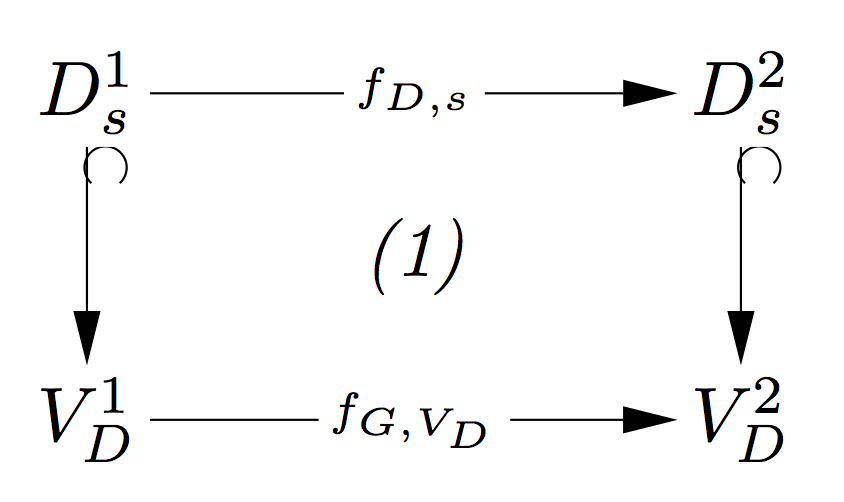
\includegraphics[width=60mm]{images/AGmorphism.png}
%\caption{AG }
\label{AG morphism}
\end{figure}

\end{ProposalDef}

For defining the Typed attributed Graph we need to first define the concept of final $D_{sig}$-algebra for a given algebra. final $D_{sig}$-algebra for an algebra is mapping somehow the name of the sort as a set to the sort as its interpretation. So cardinality of the interpreted sorts would be 1 for all of them. It maps the constant symbol of sort $S_i$, to the singleton member of corresponding carrier set $Z_{S_i}$, and following that, interpret the result of a function application on carrier set to the corresponding singleton member of the result sort.  
%:Key Def6 (final D_sig-Algebra)
\begin{ProposalDef}
Given a signature $SIG = (S, OP)$ , the \textbf{final $SIG$-algebra Z} is defined by $Z=(S_z, C_z, OP_z)$ where:

\begin{itemize}
	%\item $S_z = D_k$ where  $D_k=\{k\}$ for each sort $k \in S$;
	\item $S_z = D_s$ where  $D_s=\{s\}$ for each sort $s \in S$;
	%	\item $C_z = s \in Z_s$  for a constant symbol $c_s: \rightarrow s \in OP$;
	\item $C_z = k \in D_s$  for a constant symbol $c_s: \rightarrow s \in OP$;
	%\item $op^I : \{s_1\} \ldots  \{s_n\} \rightarrow \{s\} : (s_1 ... s_n) \mapsto s$ for each operation symbol $op:s_1 ... s_n \rightarrow s \in OP$
	\item $OP_z : \{s_1\} \ldots  \{s_n\} \rightarrow \{s\} : (s_1 ... s_n) \mapsto s$ for each operation symbol
$op:s_1 ... s_n \rightarrow s \in OP$
 \end{itemize}

\end{ProposalDef}


%%:Key Def6 (Typed Att Graph)
%\begin{ProposalDef}
%an \textbf{Attributed Graph Morphism}  $f : AG^1 \rightarrow AG^2$ for two AG graphs $AG^1=(G^1,D^1)$ and $AG^2 = (G^2,D^2)$ is a pair $f=(f_G,f_D)$ with an E-graph morphism $f_G : G^1 \rightarrow G^2$ and an algebra homomorphism $f_D : D^1 \rightarrow D^2$ such that diagram (1) commutes for all $s \in S'_D$, where vertical arrows are inclusions:
%
%\begin{figure}[ht!]
%\centering
%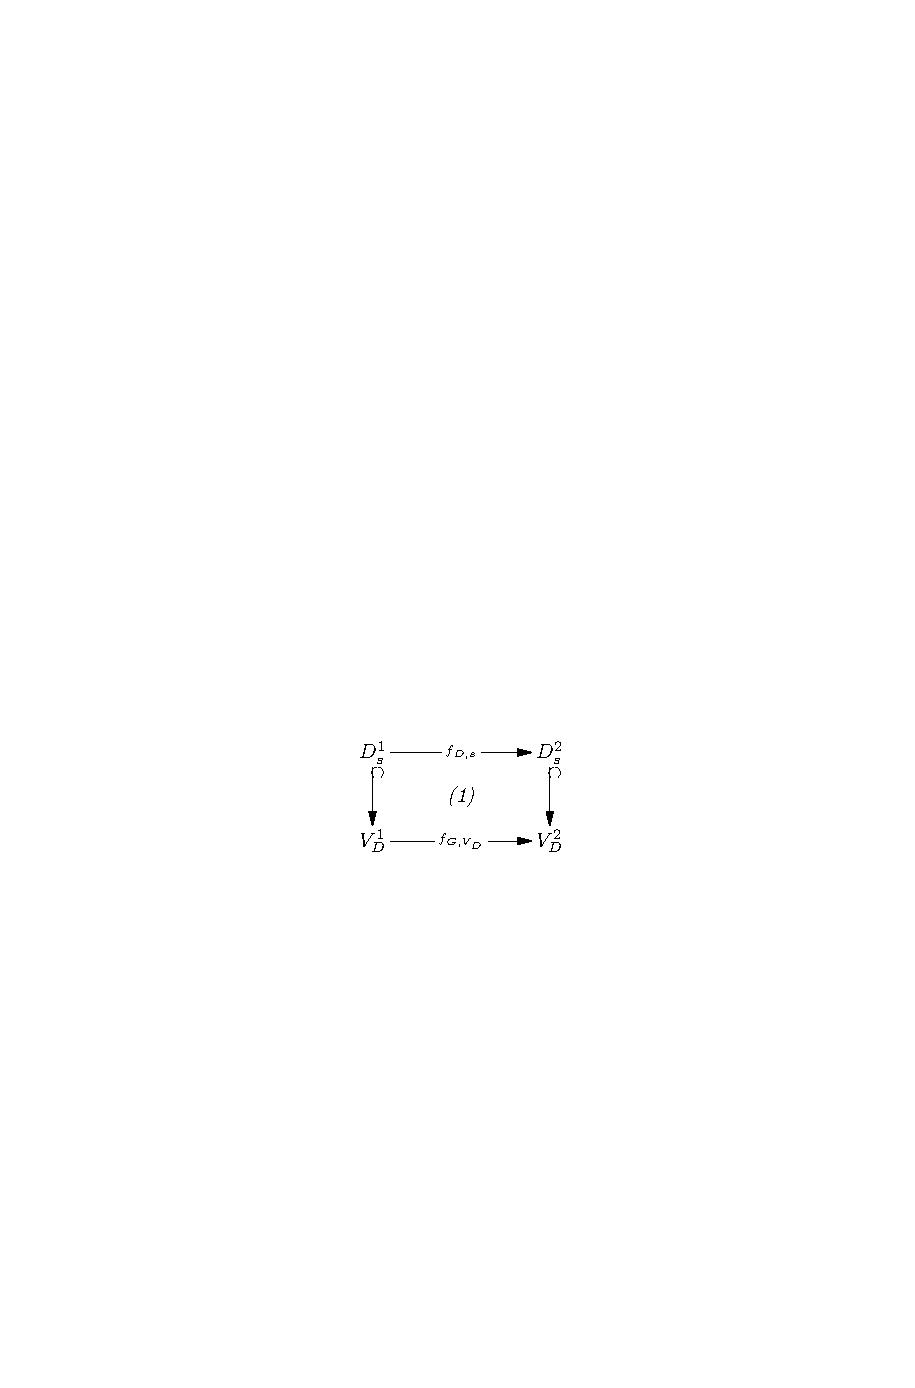
\includegraphics[width=60mm]{images/AG-morphism}
%%\caption{AG }
%\label{AG morphism}
%\end{figure}
%
%\end{ProposalDef}

%:Key Def (Attributed Type Graph(ATG))
\begin{ProposalDef}
Given a signature $SIG = (S, OP)$ , an \textbf{Attributed Type Graph(ATG)} is an attributed graph $ATG=(TG,Z)$ where Z is the final $SIG$-algebra. 
\end{ProposalDef}

So for having an Attributed Type Graph as a Type of another Attributed Graph, we need to somehow specify the typing of the 
Attributed Graph Data Structure(Data Algebra) too. That is why we need to define a final $Sig$-algebra. Typing of the Attributed Graph Data Structure is represented by the final $SIG$-algebra of the corresponding Data Signature. In the following we define Typed Attributed Graph (TAG).

%:Key Def (Typed Attributed Graph)
\begin{ProposalDef}
\label{Def:TAG}
A \textbf{Typed Attributed Graph(TAG)} over $ATG$ is defined as $(AG, t)$  where $AG$ is an attributed graph and $t$ is an  attributed graph morphism from $AG$ to $ATG$
\end{ProposalDef}


Please observe that the data-signature of of the Attributed Type Graph and Typed Attributed Graphs, Typed over that would be the same, as the definitions above implies.

\begin{ProposalDef}
A \textbf{TAG morphism} between $TAG^1=(AG^1,t^1)$ and  $TAG^2=(AG^2,t^2)$ i.e. $f: TAG^1 \rightarrow TAG^2$ is an Attibuted Graph Morphism(AGT morphism) $f: AG^1 \rightarrow AG^2$ such that $t^2 \circ f=t^1$:
\end{ProposalDef}

\begin{figure}[ht!]
\centering
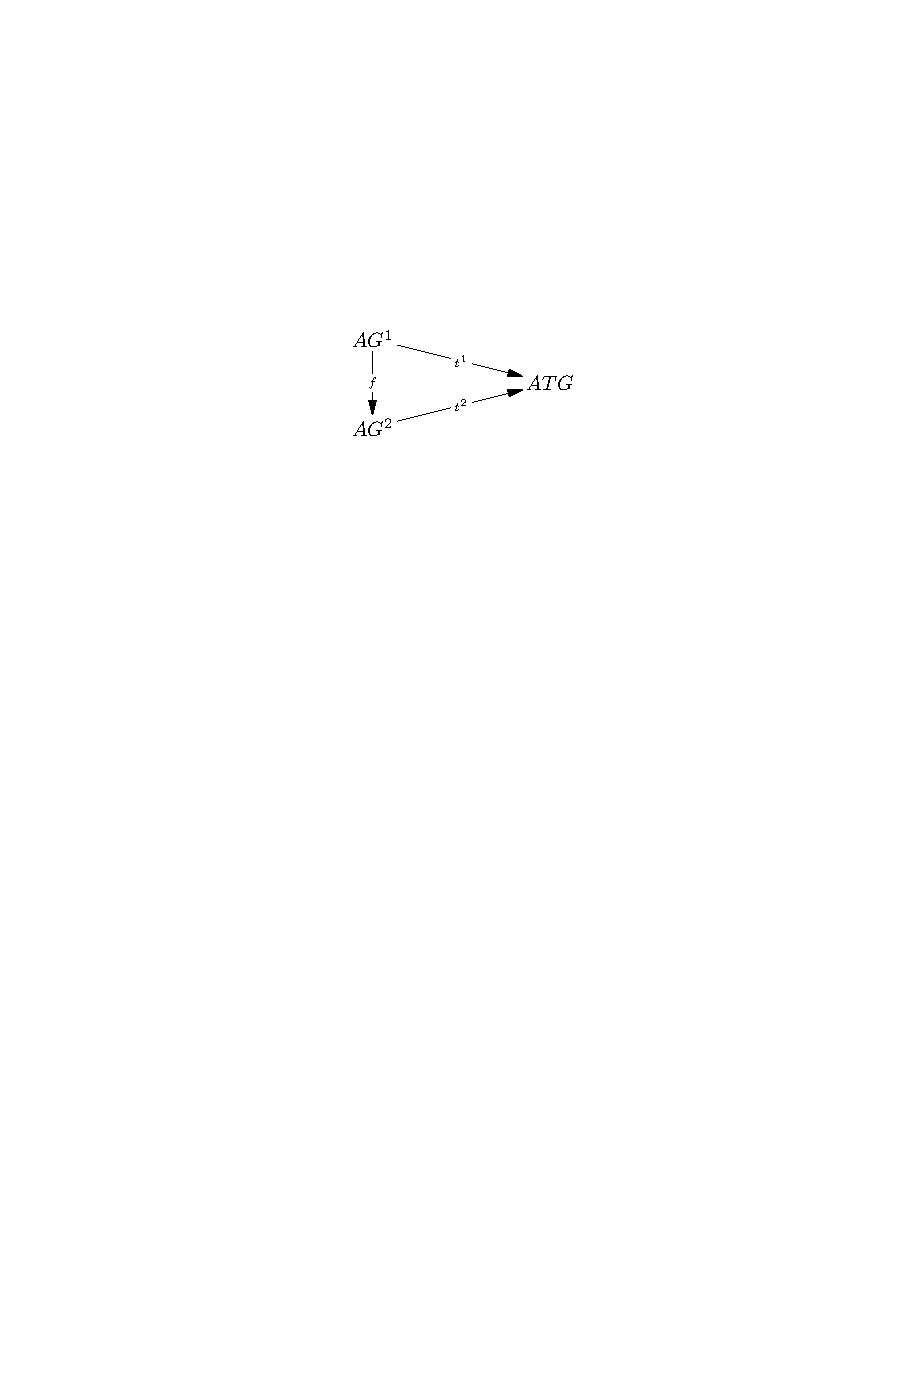
\includegraphics[width=60mm]{images/TAG-morphism}
%\caption{AG }
\label{AG morphism}
\end{figure}

In terminology of the Software Engineering, {\em Models} are equal to {\em Typed Attributed Graphs} and {\em Meta-Models} are equal to {\em Attributed Type Graphs}. This can be extended to more than one level, while meta-meta-model would be Attributed Type Graph for Attributed Type Graph of its beneath level as a Type. We should observe that all the {\em Entities} (Including Models, Meta-Models and Meta-Meta-Models) are Attributed Graphs, and the Data-signature of the connected {\em entities} by typing association(Typing Mapping) would be the same. In another word data-signature of the Model, Meta-Model and Meta-Meta-Model, all, would be the same.

\subsection{3-Dimension of Synchronization Scenarios} \label{subsec:SynchScen}
In this section we describe the three dimensions of the synchronization scenarios, including {\em Information Symmetry}, {\em Incrementality} and {\em Concurrency}, and discuss that they are orthogonal(independent) to each other, in the sense that each is describing an independent aspect of the synchronization scenario. The extended version of these dimensions are discussed in our recent submitted paper in \cite{ICMT Paper with Zinovy}. we assume two model spaces(set of models) \textbf{A} and \textbf{B} and they are supposed to be aligned(consistent) w.r.t. a relation \textbf{R}. It should be mentioned that we assume the more common cases of synchronization which only two models are involved.

\subsubsection{Information-Symmetry} captures that if two models are informationally symmetric or asymmetric. In the asymmetric case, Model A information can be completely derived by Model B. it means that having just model A we can get the model B uniquely; e.g. in common table-view scenario \cite{Bancilhon:UpdateDB:1981kx, Johnson:ConstentComp:2008vn}  view content is completely derivable from the corresponding table content. In Symmetric case neither A, nor B can be informationally derivable from each other. e.g. Class Diagram and Sequence diagram neither can be derivable from each other uniquely. Another perspective of looking at Asymmetry and Symmetry cases can be based on {\em Private} and {\em Shared} parts of the A and B. In {\em Asymmetric} case A has its own {\em  private} and {\em shared} part and B only consist of a shared part, and the private part would be empty. In {\em Symmetric} case, neither of private and shared parts for A and B are empty (ref. Figure \ref{fig:Private-Public}) The latter case is  the more general case of the synchronization scenarios in practice. \hl {Formalization of this private and public part would be the main contribution of this PhD thesis which is discussed in more details in Section {\ref{sec:Problem}}.} There is a especial case that both private parts of A and B are empty, this is called the {\em informationally bijective} case. In these cases two models are informationally equal but differently represented.
Three cases of information Symmetry is summarized in table bellow:

%:Key private-shared Picture
 \begin{figure}[ht!]
\centering
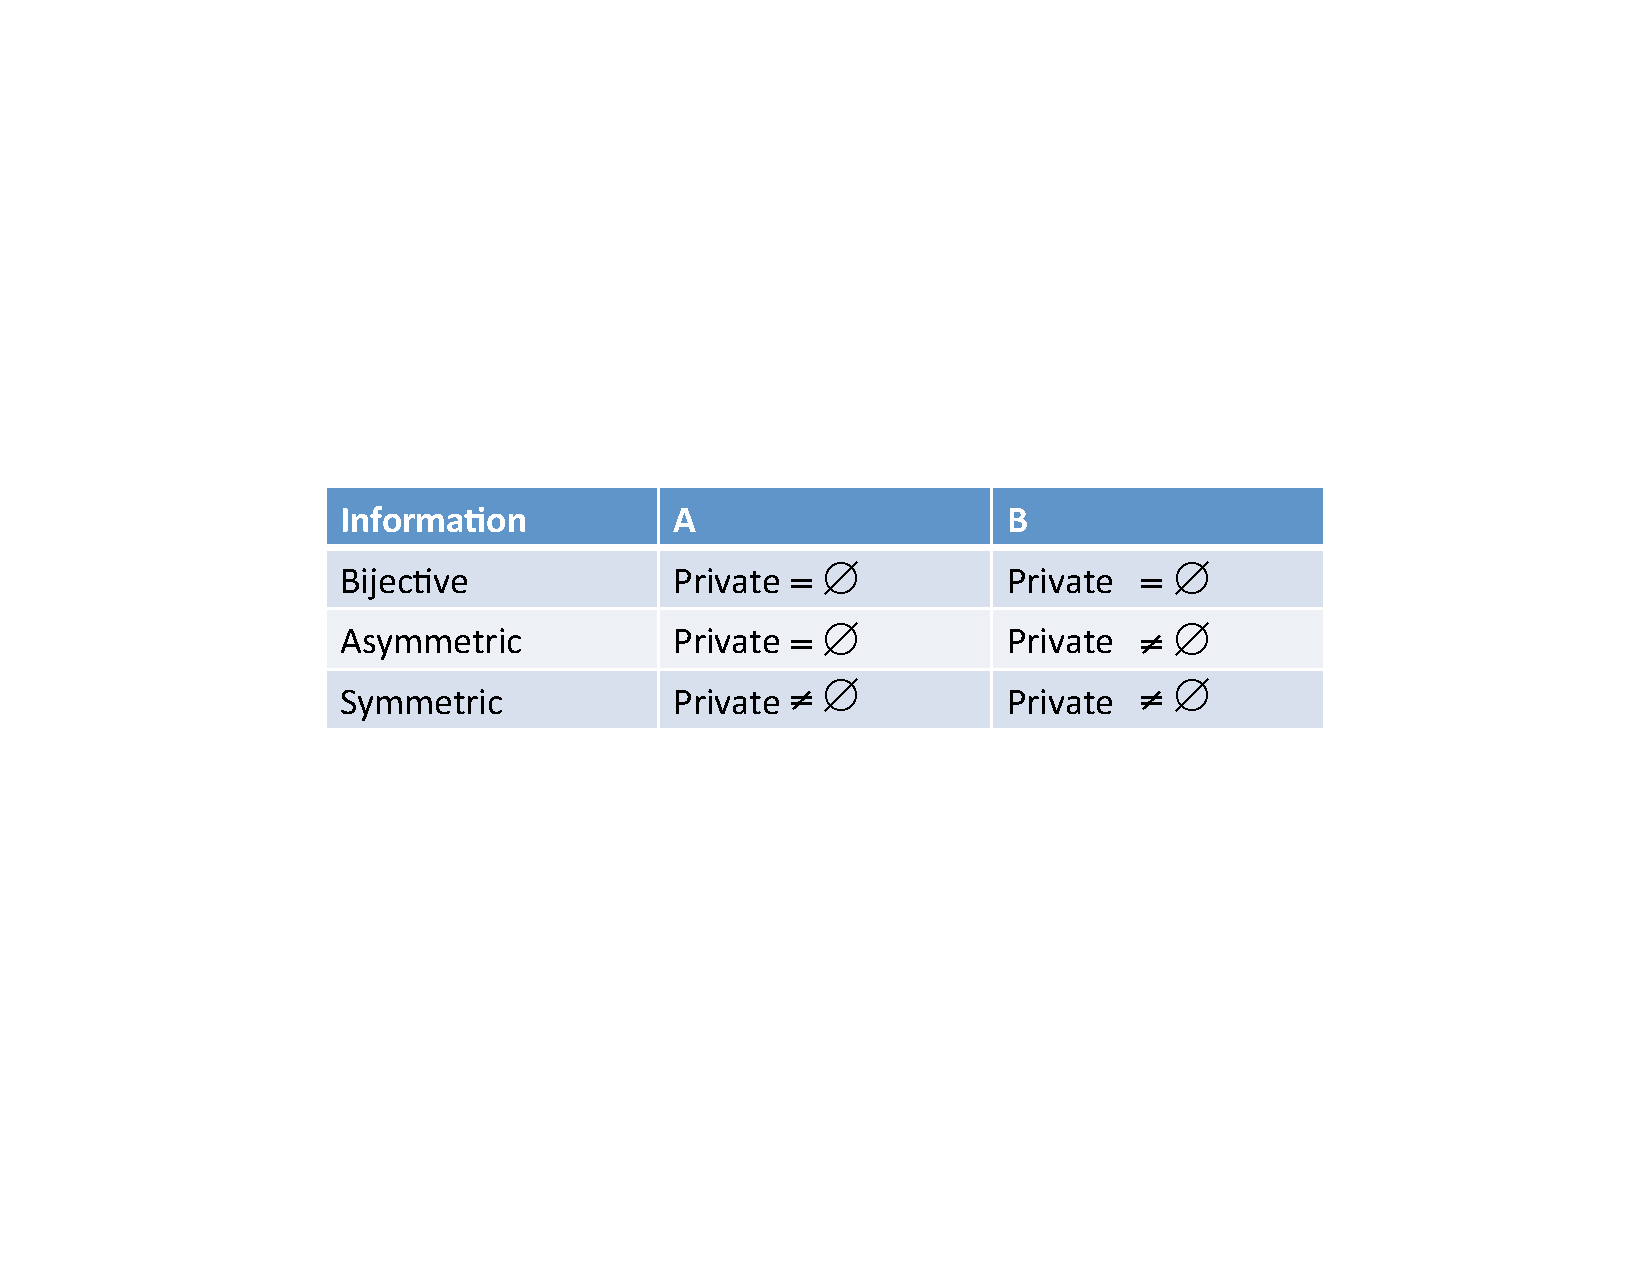
\includegraphics[width=100mm]{images/Private-Shared-Table}
\caption{Private and Shared Parts in Information Symmetry}
\label{fig:Private-Public}
\end{figure}

%a rough idea of defining a private part for Model A would be that, for any changes of the model B, you don't need to change private part to make both A and B consistent. But this idea need to be more invetigated in terms of Typed Attributed graphs.


\subsubsection{Incremetality} \label{Incremetality} of the Synchronization can be divided into three cases in terms of its maturity of the method. These three categories are called {\em Batch-update}, {\em State-based} synchronization and {\em Delta-based} synchronization. In the {\em batch update} model B is completely calculated from scratch whenever changes happen in model A. This naive strategy is not efficient at all in large model spaces $-$which are usually the case of synchronization application in practice, since for any even small changes on Model A, considerable effort is imposed on the synchronization mechanism to calculate the Model B. That is why it is usually used in small scale scenarios like type hierarchy update of a Java code \cite{ antkiewicz2008:DesigndSpace}. Propagation function in this approach accepts  $A'$ (Changed $A$) as the mere input, and generates consistent $B$ out of that from scratch. In comparison, state-based synchronizer takes $A'$ and $B$ as inputs, trying to apply the {\em Minimum Changes}  to $B$ and make it aligned with $A'$. This is far better than the previous case and commonly is referred to as {\em Incremental synchronization}. It is shown in \cite {Diskin:AsymmDelta:2011} that taking $A'$ and $B$ (states of the models) is not always enough in reconstructing the alignment between two models efficiently. So the more mature way of incrementally approach is providing the {\em Deltas}(Updates) as inputs $-$rather than states, for the propagation function. we refer to the latter case as {\em Delta-Based} synchronization. 


\hl{In both} {\em State-based} and {\em Delta-based} cases of synchronization it is not yet clearly formalized, what would be the {\em Minimum Change} as mentioned in previous  paragraph. This is another place that this thesis aims to contribute.This idea is closely related to the {\em private} and {\em public} part concepts. Since for example we need that the synchronizer doesn't change the {\em private} part of B at all and changing of the {\em shared} part of it be minimal when we say {\em Minimal Changes} on B.


\subsubsection{Concurrent} synchronization means that if two models are allowed to evolve concurrently or not. when we state that a synchronization is not {\em Concurrent}, we mean that Models $A$ and $B$ can not be changed simultaneously. It another word, if Model $A$ is evolving to $A'$ we need to first propagate its changes to $B$ and later on, evolution of Model $B$ would be allowed. In implementation it would mean that if even both models evolve simultaneously, we would give more importance on changes of one model and taking it as as {\em Master} (say $A$), while ignoring the changes of the other(Say $B$) and trying to make them aligned again. In comparison,  in {\em Concurrent} scenario, simultaneous changes to the models are allowed and both model changes are taken into consideration in the alignment process. It means that synchronization framework tries to make the {\em Minimum Changes} on evolved Models $A'$ and $B'$ to produced the new aligned Models $A''$ and $B''$. The later case is more mature and the most desirable case of synchronization.

\subsubsection{Orthogonality of the three aspects} --{\em Information symmetry}, {\em Incrementality} and {\em concurrency}, is somehow clear from the previous paragraphs. For each cases of information symmetric and asymmetric and bijective, and also for every case of {\em batch-update}, {\em state-based} update and {\em delta-based} update, we would have two possibility of concurrent and non-concurrent case. Also being {\em Information symmetric}, {\em asymmetric} or {\em bijective} doesn't depend on the approach of the incrementality. Hence we would have three orthogonal dimension in synchronization scenarios which give rise to 18 different cases in synchronization framework. Figure \ref{fig:SynchTypePic} demonstrate 9 different types. We omit the {\em concurrency} dimension for simplifying the picture. Considering two cases of concurrency all cases would double.

%:Key Synchronization Types Picture
 \begin{figure}[ht!]
\centering
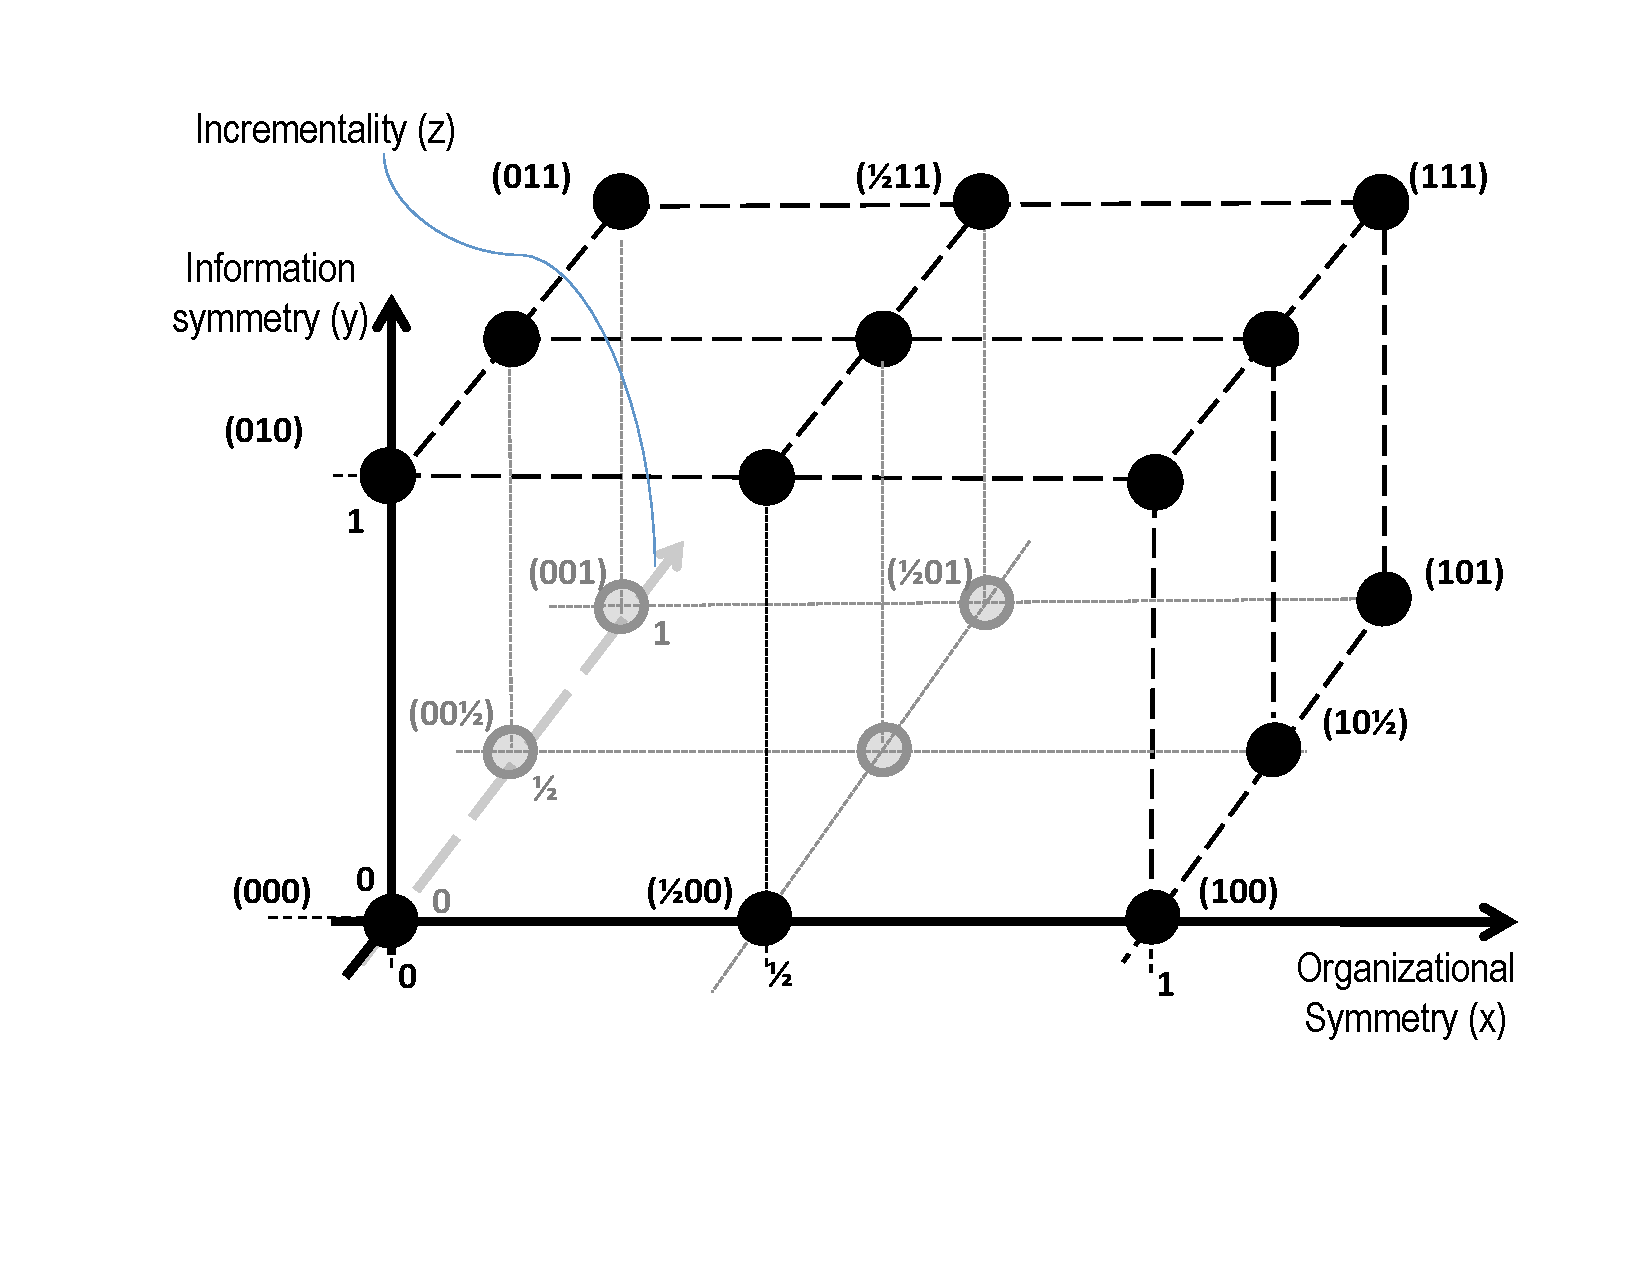
\includegraphics[width=150mm]{images/Synchronization-types}
\caption{Different Synchronization Scenarios}
\label{fig:SynchTypePic}
\end{figure}


\subsection{Pair of Transformers and Bidirectional Transformation Languages}
When we Transfer one model(say A) to another Model(say B) by writing a so-called {\em forward} transformation, we usually desire to have a {\em backward} counterpart which transfers B to A. To make our discussion more abstract, suppose that there is a Relation $R$ between $A$ and $B$ as a set of Models, and {\em Pair of Transformers}({\em forward} and {\em backward})  which are in accordance with this Relation\footnote{\label{note1}By in accordance we mean holding some properties like {\em Correctness}, {\em Completeness} and etc. which is defined later. {\em Correctness} property is necessarily basic one and should hold for all pairs of transformers.}. Often in practice the R is not explicitly defined and just the transformers is defined using some transformation languages. For example languages like {\em ATL} \cite{Jouault:2008:ATL}, {\em Viatra2} \cite {Balogh:2006:Viatra2}, {\em QVT-O} \cite{OMG:QVT:2011} or even Regular programming languages like {\em Java} are used for writing Transformers. In these situations getting a backward transformation is not trivial and oftentimes requires the user to code the backward transformation in hand. It is often desirable that these {\em forward} and {\em backward} transformers be consistent \footnote{ refer to footnote \ref{note1} at page \pageref{note1}} \cite{Diskin:DeltaSymm2011kl, Foster:LensCombinators:2005tg, steven:QVT-Semantic2010} and maintaining the consistency in pair of separate transformers which is both coded by the user is not easy and straight forward. That is why the concept of the {\em Bidirectional Transformation Languages(BX)} in which {\em Consistent} transformers can be extracted automatically out of one transformation specification is emerged. This specification in {\em BX} is somehow more explicitly specifying the Relation R between A and B. For example {\em QVT-R} \cite{OMG:QVT:2011}, {\em Triple Graph Grammars(TGG)} \cite{Schurr:1995:TGGIntro}, {\em Lenses} Framework \cite {Foster:LensCombinators:2005tg} and {\em GroundTram} \cite{hidaka2011:Groundtram} frameworks are providing {\em BX} facility. From the aforementioned frameworks, only TGG works on TAG\footnote{ refere to Definition \ref {Def:TAG}}. Table below summerises which datastructure they support as a models:


%:Key BX Framework Table representation
\begin{center}
\begin{tabular}{|c|c|}
\hline 
\textbf{Framework} & \textbf{Model Representation}\tabularnewline
\hline 
\hline 
QVT-R & UML Meta-Model\tabularnewline
\hline 
TGG & Typed Attributed Graph\tabularnewline
\hline 
GroundTram & Labeled Graph\tabularnewline
\hline 
Boomerang & String\tabularnewline
\hline 
\end{tabular}
\end{center}

Although having BX is desirable but in theory and practice there are some obstacles in making them applicable : (1) Semantic of extracting a consistent backward transformation is not trivial, (2) There doesn't exist yet a rule of thumb what is the appropriate collection of properties for the pair of transformers in different application domains (ref.  Subsection \ref{Synch:Prop})(3) Writing a transformer in BX languages like QVT-R is more complicated and tricky for the user  than writing the same transformer in one-directional transformation languages.


Out of aforementioned frameworks for the BX, each one has its pros and cons, but non is yet gained the maturity enough to be widely used in industrial cases. \hl{Out of those, since TGG are supporting TAG, we will discuss that in .... in more detail and will examine its specifications in Sec...}

\hl{(You can Write a section on TGG and formally define it and discuss it formally and say its strenghes and weeknesses)}

Now write down properties name and define them:

\section{Consistency properties of transformers}
It is desirable that pair of transformers(forward/backward) satisfy some consistency properties. For Example {\em Correctness} of the transformers is the rudementary requirement which insures that transformers operate correctly. Other consistency properties like {\em Completeness}, {\em Hippocraticness}, {\em Undoability} and {\em Invertability} are also discussed in this Section. When we talk about model {\em Synchronization} we desire that the corresponding transformers become consistent, where the consistency of the transformers is defined as conforming to subset of the following properties depending on the domain of the synchronizer application. First we define the Correctness property.
\subsection{Correctness}
\label{Synch:Prop}
%We define the notion of the Correctness in a abstract way here, and later on we would make it concrete for each of the types specified in Section \ref{subsec:SynchScen}. 
Let's call {\em forward} and {\em backward} Transformers $\overset{\rightarrow}{R}$ and $\overset{\leftarrow}{R}$ consequently supposing that they are total functions, and suppose that Relation $R$ is a desirable relation between two Set of Models(Meta-Models) $A$ and $B$. {\em Correctness} property as it is expected, simply ensures that a {\em Pair of  Transformers} are functioning correctly.

%:Key Correctness
\begin{ProposalDef} \label{CorrectnessDef}
A Pair of Transformers  ($\overset{\rightarrow}{R}$, $ \overset{\leftarrow}{R}$) are \textbf{Correct} w.r.t. $R \subseteq A\times B$, if  $(a,\overset{\rightarrow}{R}(p_1)) \in R$ and $(\overset{\leftarrow}{R}(p_2),b) \in R$ where $p_1$ and $p_2$ are set of input parameters.
$p_1$ for {\em Batch-update}, {\em State-based} and {\em Delta-based} cases(ref. \ref{Incremetality}) are $\{b\}$, $\{a,b\}$ and $\{\Delta a,b\}$ consequently where $a,a' \in A, b \in B$ and $\Delta a=(a,\Delta,a')$ for $\Delta $ being a mapping between elements of $a$ and $a' $.  $p_2$ is defined the same way as $p_1$ if we interchange $a$ and $b$ in $p_1$. 
\end{ProposalDef}
This property is defined in \cite{steven:QVT-Semantic2010} and \cite{Diskin:AsymmDelta:2011} for two latter cases of {\em Information Symmetric} cases. In \cite{Bohannon:2008:Boomerang,Hofmann:2011:SymLens} this property is defined for {\em Information Asymmetric} and {\em State-based} Cases.  

\subsection{Hippocraticness, or �check-then-enforce�} 
This property states that the transformers should not cause any change if two models are already consistent w.r.t. R. 
 
 %:Key Hippocratic
\begin{ProposalDef}
A Pair of Transformers  ($\overset{\rightarrow}{R}$, $ \overset{\leftarrow}{R}$) are \textbf{Hippocratic} w.r.t. $R \subseteq A\times B$, where  $\forall a \in A$ and $\forall b \in B$: if $(a,b) \in R$  then $\overset{\rightarrow}{R}(p_1)=b$ and $(\overset{\leftarrow}{R}(p_2)=a)$
\end{ProposalDef}

$p_1$ and $p_2$ are defined like the Definition \ref{CorrectnessDef}. The above property is called {\em "check-then-enforce"} in QVT-R specification \cite{OMG:QVT:2011}

\subsection{Undoability}
Undoability is introduced by Steven in \cite{steven:QVT-Semantic2010}. That means if we undo the changes of the $A$, any changes that happened on $B$ because of synchronization, should be rolled back to exactly its original state. We define this property for {\em State-Based} scenario as we would see it is trivial for {\em Batch-Update}. 

\begin{ProposalDef}
A Pair of Transformers  ($\overset{\rightarrow}{R}$, $ \overset{\leftarrow}{R}$) are \textbf{Undoabe} w.r.t.  $R \subseteq A\times B$, where  $\forall a,a' \in A$ and $\forall b,b' \in B$: if $(a,b) \in R$  then $\overset{\rightarrow}{R}(a, \overset{\rightarrow}{R}(a',b))=b$ and $\overset{\leftarrow}{R}(\overset{\leftarrow}{R}(b',a),b))=a$ 
\end{ProposalDef}

For the {\em batch-update} case this property is trivial and holding all the times, since we assume that the transformers are functions, then rolling back $a'$ to $a$ and executing the $\overset{\rightarrow}{R}$ on that we are obviously expecting to get $b$ again. However according above definition this might not be the case for the {\em State-based} or {\em Delta-basdd} scenarios.

It is arguable that this property is suitable to be imposed on the {\em Synchronization Implementation Environment} rather than the Synchronization {\em Transformers}.  Since at the moment {\em undoability} is well supported by modelling environments, while we believe imposing {\em Transformers} to support that would be more restrictive.

\subsection{Invertability}
It is informally means that starting from one model and going forward and backward by transformers, we will end up with the same model. In another word it states that the {\em forward} and {\em backward} transformers are the inverse of each other functioning in reverse directions. We define invertability for the {\em State-based} cases, and for the rest it would be the same.  Following definition is adopted from \cite{Zinovy:2008:AlgForSynch}.

\begin{ProposalDef}
A Pair of Transformers  ($\overset{\rightarrow}{R}$, $ \overset{\leftarrow}{R}$) are \textbf{Invertabe} w.r.t.  $R \subseteq A\times B$, if  $\forall a,a' \in A$ and $\forall b,b' \in B$:  $\overset{\rightarrow}{R}(a, \overset{\leftarrow}{R}(a,b',b),b)=b'$ and $\overset{\leftarrow}{R}(b, \overset{\rightarrow}{R}(a,a',b),a)=b'$ where $\{(a,b),(a',b')\} \subset R$ 
\end{ProposalDef}


\subsection{Completeness}
Completeness says if there exists at least one model, say $b$, which is in Relation with Model $a$, then transformer should be able to transform $a$ to it. In another word {\em Completeness} states that the transformers should be total functions and return nonempty in the case there is a counterpart for its input(s) regarding relation R


\begin{ProposalDef}
A Pair of Transformers  ($\overset{\rightarrow}{R}$, $ \overset{\leftarrow}{R}$) are \textbf{Complete} w.r.t.  $R \subseteq A\times B$, if $\forall a \in A,  \overset{\rightarrow}{R}(a)\neq \emptyset$ if $\exists b \in B$ where $(a,b) \in R$  and if $\forall b \in B,  \overset{\leftarrow}{R}(b)\neq \emptyset$ if $\exists a \in A$ where $(a,b) \in R$ 
\end{ProposalDef}

\section{Literature Review} 
\label{sec:Lit}
Talking about Model Synchronization, we already tied with all other aspects of MDE concepts including : {\em Model Transformation}, {\em Meta-Modeling}, {\em Model Specification Language}, {\em Constraint} and {\em Bidirectional Model Transformations(BX)}. At the moment there are many research activities progressing in each area independently and inter-relatively. 

% Talk about BX
% you can cite crystoph fwork on bidirectional transfo *(japan paper), steven on lanscape of bx
%Cite QVT and semantic issues
%Cite lense word
%Cite boomerang and ground tran
%Cite zinovy paper on algebraic approach on Synch and also Delta lenses
Considering {\em Models} as {\em Graphs}, {\em Graph Transformation} Techniques are considered as a {\em Model Transformation} foundation in that sense. The book in \cite{book:Rozenberg1997} discusses Graph Grammar and DPO(Double Push out) and SPO(Single Push out) approaches as two well-known specification for {\em rule application} definition in Graph Transformation . Another book \cite{book:Ehrig2010} discusses some algebraic foundations of graph transformation using Category Theory \cite{Barr:CATBook:1999dz, Awodey:CATBook:2009fv}. These two books are providing informative materials in domain of Graph Grammars and Graph Transformation which are closely related to model specification and model transformation basics respectively. Attributed Typed Graph(ATG) are introduced in \cite{Ehrig:2006:OverviewOfFormalConcept} as a formal representation of Models. There are some alternatives for ATG specification which are also discussed in \cite{ other approach of Attributed typed graph}.


There are many research at the moment progressing on {\em Graph Transformation} and also some academic tools have been implemented for them. \cite {you might want to put some ref like Atom3, AGG, and some other tools}. Among them {\em Triple Graph Grammars}(TGG) as an extension of regular Graph Grammars and their tools holds more than 15 year research background \cite{Schurr:2008:15Years} and some successful application \cite{ you can cite some TGG application here!!}. TGG rules are specifying source and target model evolution in a constructive manner. It is introduced by Andy Sh\"{u}re  in \cite{Schurr:1995:TGGIntro} and formally defined in \cite{Konigs:2006:TGGFormalDefSetBased}, \cite{Ehrig:2007:IPB:TGGFromalDef} and \cite{Golas:2012:TBG:TGGRecentFormalDef} recently. TGG approach is taking Graph Grammars as a Triple of {\em Source}, {\em Correspondence}, and {\em Target} Models and defining the relationship between them as a Triple Graph Grammar Rules \cite {Kindler2007:TGGConcepts}. TGG is considered as a Graphical Bidirectional Transformation Languages (BX) too, which forward and backward rules can be extracted from the {\em Triple Rules} in a straight forward manner \cite { Put kindler paper ref here}. Some properties of 
 of TGG like {\em Functional Behaviour}, {\em Correctness}, {\em Completeness}, and {\em Termination} are formally studied here \cite {Hermann:2010:FAF:FunctionalBeh, Ehrig:2009:OCC:OnTheFly, Ehrig:2008:RMT:OnTheRel}. 
 % talk about TGG Tools
Besides the Theory of the TGG there are some tools developed for that in academia and some of them applied successfully for industrial projects \cite{ Giese tool applied, I think he has a long paper describing this}. Among these we can mention MoTE \cite{giese2012:Bridging}, eMofelon \cite{anjorin2011:emoflon}, TGG Interpreter \cite{greenyer2008:TGGInter} and Emorf \cite{klassen2012:emorf}. Although Bi-directionality of the TGG provides some advantages over its usage in term of providing the consistent forward and backward rules for granted, at the same time its usage is limited in defining complex transformation scenarios which are demanded in most industrial cases \cite{ cite paper that compare Trans models and Reject TGG}. Besides there are still some space left for research to formalize the application of {\em Constraints} in rule definition which is necessary to use in most of its applications \cite{ try to cite something related to constraint on TGG here}.



Giese and Wagner discuss incremental model synchronization implementation in TGG in \cite {giese2009:IncrementalSynch}; But no formal foundation is provided to verify how far their incremental implementation is correct in the sense of being {\em Incremental}. This is actually one of the objectives of this PhD research to establish a mathematical specification which incrementality of the synchronization can be verifiable. \hl{Regarding Synchronization Techniques in TGG, {\cite{hermann2012:concurrent}} studies Conflict Resolution strategies in TGG approach. (Maybe you need to read that paper and put some comments here).}

% cite some other transformation languages.
Lenses Framework is discussed in \cite{Hofmann:2011:SymLens}. It is trying to provide a consistent forward and backward transformation out of single specification language. Boomerang framework \cite {Bohannon:2008:Boomerang} is implemented based on that idea. But the language application is limited to the String Type of Data at the moment and covers the Asymmetric cases in Synchronization Scenario. There is no discussion on the incremental update integration to the framework and the emphasize in on defining BX language. 
GroundTram \cite {hidaka2011:Groundtram} is another thrend trying to define a BX programming languages based on edge-labeled Graphs. They are using $UnQL^+$ language(an Extension of UnQL \cite{buneman2000:UnQL} ) for defining the Bidirectional Transformation, but again the emphasize is on the Bidirectionality rather than the incrementality.

(Should read Zinovy Tile Algebra paper and also Algebraic approach to comment on that)
(I also need to read xiong paper on incremental approach and comment on that)
(I also need to read TGG sychronization of Ehrig and Zinovy and comment on that) 

% cite crystoph work on Synch  
Shynchronization scenarios is categorized in eighteen different categories in \cite{antkiewicz2008:DesigndSpace} 

%Cite Xiong work on Synchronization





%Does it necessary to study synchronization and cuncurrent synchronization in BX domain? It seems no!
%you can take it in a unidirectional domain and study that in that ares, I think there should be some text on th e lirature which covers this topic. for example you wrote a transfo. on ATL from A to B, then A changes, so how to propogate tis change to B, not touching unrelated data. That arise the fact that how to extract unrelated data from just unidirectional transformation. In another world How we can get  the relation R from just undirectional case, in the sense that we almost consider Transfo as a function, so it means that the R is a function. This is not realistic!! in practice , we define Transfo, as a function, but taking the shared part of the target as domain. in that sens yes that is function. but that dosn't mean that whole design space of the Target make that transfo a function. let say an example: we define transfo from class diagram to code : this is function, Does the relation from class diagram to code is function? No,  Why? --> because for one class diagram there are many implementations which differ in body of the class methods. so the relation from model to code in not a function. In practice we usually specify this relation as function.  So we can just examine the matter of model synchronization in unidirectional cases as a special case of bidirectional case. this gives the opportunity to study this area independent of the BX which its result can be later extended to BX.

%-----------------
ofGrapEhrig et. al discusses the fundamentals of algebraic Graph Transformation is a seriese of books, and articles. defining Attributed Typed Graph as Model, Graph Grammars and loot[Some Ref here to TGG, all ref to TGG, GroundTram, , Constraints: donloaded constraint papers, BX: Crystoph paper] . Among aforementioned Subjects the first one, Model Transformation and BX is closely coupled with Model Synchronization. At the moment there are couple of approaches [TGG, Lenses, GroundTram] , languages [Boomrang, ATL, QVT, Viatra2, and many academic tools [AGG, Emofelon, MoTE, TGG-Interpreter, Emorf, MediniQVT]  developed based on those thories and there is active research groups working on them.


\hl{ mention the tools related to TGG, TGG-interpreter, Mofelon, Gies tool, emorf, emf, japan tool, mediniQVT, smartQVT, SDM,}


\section{Problem Definition}
\label{sec:Problem}
\hl{I think it is possible to move some parts from the background to here like the space of synchronization}

Almost all Synchronization formalization is based on the assumption that we have R clearly defined by some specification constraints \cite { Zinovy Work, TGG (Check it), Xiong work }. But in real application usually R is not clearly defined especially in the complex cases of Model Transformation and Synchronization. For example in TGG Approach \cite{Ehrig:2007:IPB:TGGFromalDef, Konigs:2006:TGGFormalDefSetBased}, Relation between source and target is defined implicitly by TGG rules in constructive and operational way \cite{one of TGG papers}, or in ATL \cite{Jouault:2008:ATL}, Viatra2 \cite{Balogh:2006:Viatra2} R is defined in one direction as a function. Defining a Relation as a function is useful if the nature of the Relation be one-to-many or info-Asymmetric like the Table-View Relation in database domain \cite{cite one of table view papers here}. Apparently the backward transformation of this case would not be a function and would require an update policy to make it a function \cite { cite a update policy paper here}. There are two points regarding our latter discussion that we need to mention out here: (1) there are many cases of model synchronization that are not info-Asymmetric, so the relation definition can not be specified by a function in neither direction (both forward/backward) (2) even in the case of info-Asymmetry, we need to avoid the naive, inefficient and non-intelligence method of batch update of the target for every change that happens on the source. In both above cases (info-asymmetric and info-symmetric) we need to know two important facts: (1) which change in the source imposes changes on the target according to the defined Transformation Function or Relation. we define {\em Private parts} of the source, the entities that any change to them would not impose a change to the target as apposed to {\em Shared parts} which any changes to them requires a change to the target to satisfy the  constraints and  establish the relationship again.\hl{ As we will show by example latter}, distinction of {\em Private} and {\em Shared parts} is not trivial and straight forward result gained out of Relation or Function definitions. (2) if it is determined that the target should be changed (because of {\em Private part} change in source,) how to preserve the relationship(make the target aligned again with the source) by {\em minimum possible change} on the target. In the general case of the info-symmetry(many-to-many Relation) many possible alignments would be possible, however we are interested in one(or maybe a set) of them which are the most desirable(minimum possible change on the target). \hl{we will discuss this case more by an example later}. For addressing this problem it seems that we might need to define some measurements for the updates and calculate the most desirable updates according to these measurement. Hence we would need to identify suitable measurements according to some factors like usability and practical application of synchronization cases.
if we can address the previous problem in terms of defining a {\em Private} and {Shared parts} formally for the models based on the synchronization scenario, and also identify some criteria for the {\em desirable updates} on the target, then we can give a formal semantic for the concept of incremental synchronization. Therefore synchronization frameworks can be implemented and verified according to that semantics.


\hl{ it seems that choosing these} {\em \hl {desirable}} \hl{ changes can not be mechanized?! And they might be just user choices, but in the case that the alternatives are too much for the user to choose there should be some filters which makes them a well-acceptable set of option in some sense out of which user can select. In latter situation those filter parameters can be defined by Transformer Executer (user).}

The extended case of the incremental synchronization formalization would be the {\em concurrent} cases of synchronization which the changes are allowed simultaneously at the source and target in one step.  \hl{ should explain this more}

\hl{QVT-R {\cite{ QVT-R}} and TGG are two approaches that can be  used for Relation Definition among two models in industry, so try to demonstrate the problem by some example based on these two approaches. (What are the other Relational Languages for Relation definition among two models. )}


Steven Criticises on the QVT-R semantics!


Solution: some speculation
defining a transformation as a function is ATL and Viatra2 is easier than QVT-R, so maybe better idea to have two functions which is practical than one function and let the tool keep the properties among them in according to the constraint that user desire to be maintained by the tool. I mean give the option to the user to choose that criteria getput, hipocratic, invertability, undoable, and .... in maintained for these two functions in pair (forward/backward). since it makes the transformation writting for users easy and practical.

\hl{the following part should be commented or moved to the methodology and approach section}
( one look is that looking a the transformation functions defined in ATL and Viatra, and see how they define that function. according to that function the source is sliced into some pieces which each piece is mapped to one target . Reverse looking at this function is a kind of defining half of the full relation in a way that $t \in T $ there exist many $ s \in S$ where $s R t$ .  so out of forward transformation function (lets take it as total just by mapping non-mappable cases (not transferable cases) to null) we can get the half of the relation like $\{s_1 R t_1, s_2 R t_1,  s_3 R t_1, s_4 R t_2 , s_5 R t_3 , ...\}$, we can look at that like $\{\{s_1, s_2,  s_3\} R t_1,\{s_4, s_5\} R t_3\}$ too. Forward transformation function is not always surjective. By the reverse case (backward function) we would have the other half of R $\{ t_1 R s_1, t_2 R s_1,  t_3 R s_1,t_4 R s_2 , t_5 R s_2 ...\}$, we can look at that like $\{\{t_1, t_2,  t_3\} R s_1, \{t_4, t_5\} R s_2 ...\}$ or reverse of it $\{s_1 R \{t_1, t_2,  t_3\} , s_2 R \{t_4, t_5\} ...\}$. so the question is that if these two functions together define the desired Relation R?! I think this is closely related to the constraints that forward and backward transformation should preserve some constraints like hipocraticness(check and force), inevitability, GetPut and ....) to be a BX. They should be studied more!!!!
Another thing that come to my mind is that it can be related to meta-models too! so meta-models for sure are involved in definition of this private and shared parts.



% look at the background def. from draft file and fill out here!

\hl{you need to mention AGG tool {\cite{Taentzer:AGG:2000zr}} in your proposal! , also SDM {\cite{Fischer:SDM:2000ys}}, also EMF {\cite{Steinberg:EMFBook:2008qf}}}

\subsection{Example Demonstrating the Problem}
\hl{I should add example to demonstrate the problem with some examples.}
 Here we are going to show two examples demonstrating the issues related to the {\em Private} and {\em Shared} Parts. Look at the Figure \ref{fig:Example1Pic}. {\em People} Table(Model Space A) representing the records(Models) of People while {\em Employee} Table(Model Space B) representing Employee records. The Relation $R$ between {\em People} and {\em Employee} is that each person is related to the employee with same \verb+Name+ and the \verb+age+ : 
 
 \hl{(one tricky thing is that how to represent the example 1 Model spaces with TAG)}
 
$ \forall a\in A$ and $\forall b \in B,  (a,b) \in R$ if $a.Name=b.Name$ and $a.Age=b.Age$

According to above relation \verb+John+ and \verb+Mike+ record are related to each other.  In first look it seems that the \verb Name and \verb Age are the {\em Shared} part of {\em People} and {\em Employee} in the sense that their changes in each table will cause a change in another table. This result is also can be seen by looking at the Relation Definition above. We can say since the names of the elements(\verb+Name+ and \verb+Age+) are literally exists in the Relation Definition, so those elements are part of the {\em Shared} entities. But when we change the \verb+Bdate+ content in the {\em People}, it would also cause a change in the Employee \verb+Age+ in Employee table. So Bdate Changes should also propogate to the Employee too. That is because of internal functional dependancy \cite{Databasebook} between the Age and Bdate in People table.

Models in general sense are not as simple as records. as we showed in Section \ref{TAG} they can be formally represented by Typed Attributed Graph. The Notion of the dependancy between the data items in the record can be generalized to the cross cutting constraints between the model elements inside the Graph. So in that sens it is not trivial to distinguish the {\em Private} and {\em Shared parts} out of looking at the Relation Definition between two Models. \hl{maybe refer to another example with graphs in the following sections}.  In practice, it is also not the case that we always have a clear Relation Defintion literally between two Model spaces in terms of their elements. That is because specifying Relational dependancy between large Model is so complicated as apposed to specifying the Transformers by functions, so latter is preferred -- That is one of the reason why languages like ATL and Viatra2 gained more interest over the relational counterparts like QVT-R and TGG in industry. To this end, further investigation of specification of the {\em Private} and {\em Shared Parts} even specifically in each approach of Model Transformation and Synchronization is necessary. It is worth recalling that the this concept is demonstrating its importance while the changes on one model are so small in comparison to the whole model and we want to make the least effort in maintaining the consistency after these changes. \cite {Gies paper in incremental Graph}

Another aspect of the problem is identifying the least possible changes in the target for maintaining the consistency relation. Suppose in above example we change the Age Group in Employee table from 1 to 2. The most reasonable option for aleviating the Age and Bdate value in People Table is that reounding them to the nearest lowest and largest value to maintain the Relationship. We call this the {\em Minimum/Least Change} concept. This change is not always in terms of the values as it is in the database tables, and it needs to be defined in terms of Graph structures as of Model representatives. So this needs to be more investigated and studied in terms of Models and Model Incremental Synchronization. It is clear that probably we'd better not to limit the options of changes to exactly one cases (i.e. change Age to 60), but provide the user with a range of most probable options (i.e. 60- 70) rather than (60 - ...).

 


%:Key Example 1 Picture
 \begin{figure}[ht!]
\centering
\includegraphics[width=150mm]{images/example1}
\caption{People and Employee model spaces}
\label{fig:Example1Pic}
\end{figure}


As another example we are considering the transformation between the rail projects and the petrinet discussed in \cite{Kindler2007:TGGConcepts} using Tripple Graph Grammars \cite{sddsd}


\hl{ you can take it in a unidirectional domain and study that in that area, I think there should be some text in the literature which covers this topic. for example you wrote a transfo. on ATL from A to B, then A changes, so how to propagate its change to B, not touching unrelated data. That arise the fact that how to extract unrelated data from just unidirectional transformation. In another world How we can get  the relation R from just unidirectional case, in the sense that we almost consider Transfo as a function, so it means that the R is a function. This is not realistic!! in practice , we define Transfo, as a function, but taking the shared part of the target as domain. in that sense yes that is function. but that doesn't mean that whole design space of the Target make that transfo a function. let say an example: we define transfo from class diagram to code : this is function, Does the relation from class diagram to code is function? No,  Why?  because for one class diagram there are many implementations which differ in body of the class methods. so the relation from model to code in not a function. In practice we usually specify this relation as function.  So we can just examine the matter of model synchronization in unidirectionally cases as a special case of bidirectional case. this gives the opportunity to study this area independent of the BX which its result can be later extended to BX.}


\section{Methodology and Approach}\label{sec:Methodology}

\begin{itemize}
	\item just looking at different example of model transformation and investigating them according to the abstract classification of them done in the paper. \hl{read next paragraph}
	\item need to investigate more examples and their formal representation in AGG.
	\item need to work with AGG tool as an Algebraic graph transformation Tool.
	\item it seems that we need to study the relation between two models deeply.
	\item  It seems that the meta-models can be involved in {\em Private} and {\em Shared} part definition. But I don't know how?
	\item I think since this is gonna be practical work my approach would be examining the functional way of defining the relationship which is currently practiced in industry and is more popular.
	
\end{itemize}

One prospective approach to the problem would be trying to abstractly capturing the real worl transformation by ATL and Viatra2 and study how a transformation function on them define the Relation R. then trying to identify the private parts and shared parts in those instances. so trying for different concrete examples and trying to capture the abstract idea of private and shared part and formalising it.  this can be done for even Relational languages.

Since the formalization of the Models and Typed Models are very tied with the CAT theory, it seems that maybe some categorical patterns and concepts would help there abstracting out the concept. therefore increasing the knowlage of category theory and studing the patterns related to the Modeling and MetaModeling seems to be useful.

For the rest of 3 Month examing two Languages ATL and Viatra 2 and reading about the CAT theory pattern. seeing examples in them, matching them with the 3D space concept in the paper.

for the 2 month formalizing the idea.

the rest of 5 month publishing the thesis.

5 month gap for paper submission and tackling new obstacles identified during research which is not clear at the moment.

so within 15 month from now, thesis is gonna be submitted.




\section{Conclusion}\label{sec:conclusion}
\hl{ You are gonna put the conclusion here}

\begin{itemize}
	\item What is this paper is about?!
	\item What is the problem identified  
	\item How you gonna approach it.
	\item if you solve this what will happen (what is the contribution)
\end{itemize}





\pagebreak

% This includes all references from the BibTeX file in the bibliography
\nocite{*}

\begin{spacing}{1}
  \bibliographystyle{plain}
  \bibliography{ref-list}
\end{spacing}

%-----------This is commented Appendix Part---------------
%\appendix
%\section{Further Open Problems}
%\label{appendix:OpenProb}

\end{document}
